\documentclass[12pt,twoside,a4paper]{article}
\usepackage[hmargin=25mm,vmargin=20mm]{geometry}
\usepackage[pdfpagelabels=false,pdfborder={0 0 0}]{hyperref}
\usepackage[superscript]{cite}
\usepackage{amsmath}
\usepackage{booktabs}
\usepackage{caption}
\usepackage{graphicx}
\usepackage{multicol}
\usepackage{ogonek}
\usepackage{subcaption}
\usepackage{url}
\usepackage{xcolor}
\renewcommand{\arraystretch}{1.2}

\begin{document}

\setcounter{page}{1}

\title{\vspace{-1cm}
    {\Large CST Part II Unit of Assessment\\Data Science: principles and practice}\bigbreak
    {\bf Report on the Final Practical: Analysing Clickstream Data for Online Shopping}}
\author{Xiangyu Zhao\\Trinity College\\CRSid: xz398}
\date{3 December 2020} 

\maketitle

%\tableofcontents 

\section{Introduction}

In the final practical, I am required to analyse a clickstream dataset on an e-shop clothing website \cite{LapczynskiBialowas2013} between April and August 2008. I am required to interpret \texttt{price 2} as representing a user's potential willingness to pay a premium price, and build a predictive, machine learning model to predict the target value -- \texttt{price 2}, so that in the future the website can be dynamically altered based on the user or their behaviour, in order to maximise profit.
%
% The dataset contains the following attributes:
%
%\begin{itemize}
%    \item \texttt{year} (2008);
%    \item \texttt{month}, from April (4) to August (8);
%    \item \texttt{day};
%    \item \texttt{order}, which is an integer representing the sequence of clicks during one session;
%    \item \texttt{country}, which is an integer representing the country of origin of the IP address, containing 41 different countries, 5 top-level domains (\texttt{*.biz}, \texttt{*.com}, \texttt{*.int}, \texttt{*.net}, \texttt{*.org}), and one category for unclassified (12);
%    \item \texttt{session ID}, which is an integer representing the session ID (short record);
%    \item \texttt{page 1 (main category)}, which is an integer representing the main product category:
%        \begin{enumerate}
%            \item Trousers
%            \item Skirts
%            \item Blouses
%            \item Sale
%        \end{enumerate}
%    \item \texttt{page 2 (clothing model)}, which is a string representing the code for each  product (217 in total);
%    \item \texttt{colour}, which is an integer representing the colour of the product (14 in total);
%    \item \texttt{location}, which is an integer representing the photo location on the web page. The screen has been divided into 6 parts:
%        \begin{enumerate}
%            \item Top left
%            \item Top in the middle
%            \item Top right
%            \item Bottom left
%            \item Bottom in the middle
%            \item Bottom right
%        \end{enumerate}
%    \item \texttt{model photography}, which is an integer representing with 2 categories:
%        \begin{enumerate}
%            \item En face
%            \item Profile
%        \end{enumerate}
%    \item \texttt{price}, in US dollars;
%    \item \texttt{price 2}, which is an integer representing whether the price of a particular product is higher than the average price for the entire product category;
%    \item \texttt{page}, which is an integer representing the page number within the e-shop website (from 1 to 5);
%\end{itemize}

\section{Data Exploration}

By looking at the \texttt{info()} of the dataset, I can see that there are 165,474 records in this dataset, and satisfactorily, there is no empty entry in the dataset.

Since the \texttt{year}, \texttt{month}, and \texttt{day} attributes are separated in the dataset, I manually added a \texttt{date} attribute to the dataset that merges the \texttt{year}, \texttt{month}, and \texttt{day} attributes, setting the first day (i.e., 1 April 2008) as day 0. Since the \texttt{page 2 (clothing model)} attribute contains textual data, I encoded it into numerical values, so that I can inspect the data distribution later on.

The statistical summary of the dataset are obtained by calling the \texttt{describe()} method (excluding the \texttt{year} attribute since there is only one value):

\begin{center}
\begin{tabular}{lrrrrrrrr}
\toprule 
{} & \texttt{month} & \texttt{day} & \texttt{date} & \texttt{order} & \texttt{country} & \texttt{session ID} & \texttt{page 1} & \texttt{page 2} \\ 
\midrule 
mean & 5.59 & 14.52 & +61.68d & 9.82 & 26.95 & 12058.42 & 2.40 & 82.74 \\  
std. dev. & 1.33 & 8.83 & 40.73 & 13.48 & 7.15 & 7008.42 & 1.14 & 59.12 \\ 
min & 4 & 1 & 0d & 1 & 1 & 1 & 1 & 0 \\ 
25\% & 4 & 7 & +24d & 2 & 29 & 5931 & 1 & 38 \\  
median & 5 & 14 & +59d & 6 & 29 & 11967.5 & 2 & 70 \\ 
75\% & 7 & 22 & +98d & 12 & 29 & 18219 & 3 & 132 \\ 
max & 8 & 31 & +134d & 195 & 47 & 24026 & 4 & 216 \\
\bottomrule
\end{tabular} 

\begin{tabular}{lrrrrrr}
\toprule 
{} & \texttt{colour} & \texttt{location} & \texttt{model photography} & \texttt{price} & \texttt{price 2} & \texttt{page} \\ 
\midrule 
mean & 6.23 & 3.26 & 1.26 & 43.80 & 1.49 & 1.71 \\  
std. dev. & 4.24 & 1.71 & 0.44 & 12.55 & 0.50 & 0.98 \\ 
min & 1 & 1 & 1 & 18 & 1 & 1 \\ 
25\% & 3 & 2 & 1 & 33 & 1 & 1 \\ 
median & 4 & 3 & 1 & 43 & 1 & 1 \\ 
75\% & 9 & 5 & 2 & 52 & 2 & 2 \\ 
max & 14 & 6 & 2 & 82 & 2 & 5 \\ 
\bottomrule
\end{tabular} 
\end{center}
\bigbreak
The data distribution histograms of the attributes are also plotted:
\medbreak
\begin{center}
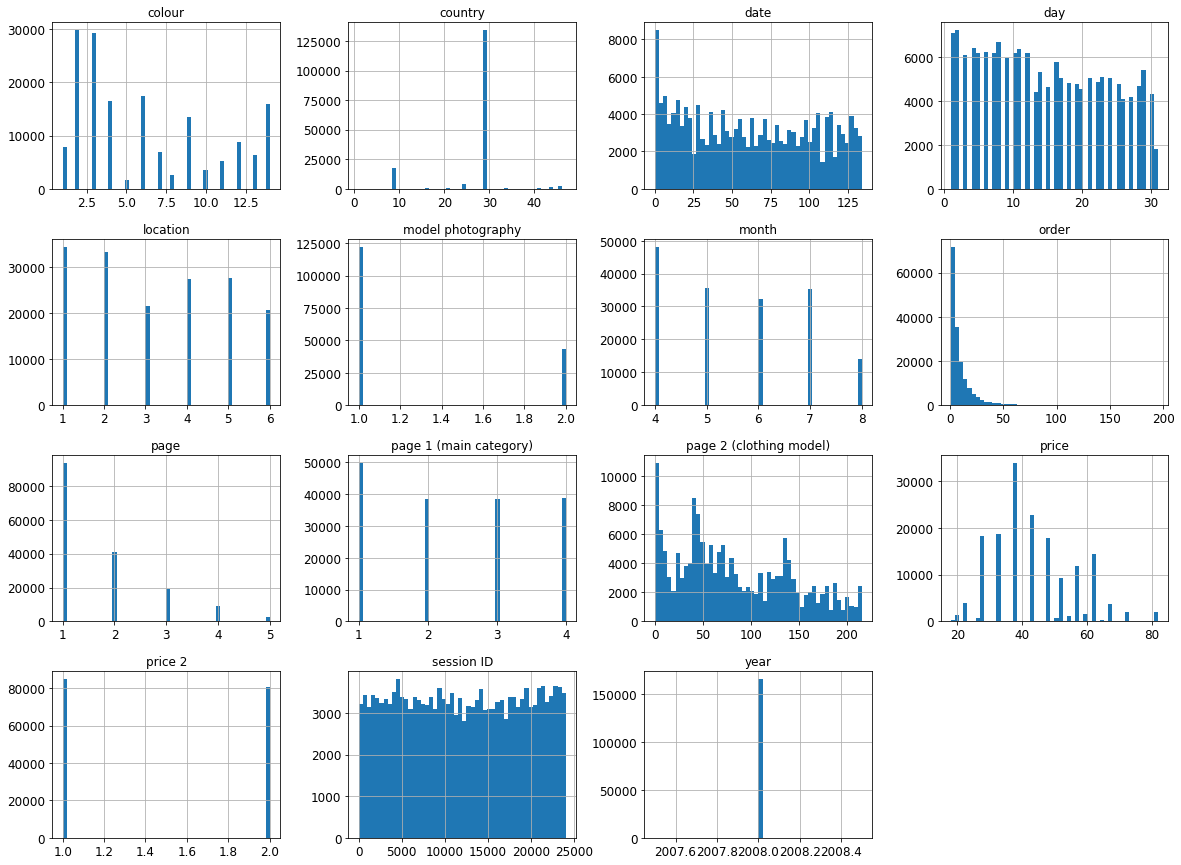
\includegraphics[width=\linewidth]{images/histogram.png}
\end{center}

By looking at the data distribution, the following findings can be obtained:

\begin{itemize}
    \item Other than the first few days in April 2008 that has a lot more clickstream records, the number of clickstream records in the rest of the dates within the interval of this dataset are roughly at the same level, though there might be some periodic peaks and troughs;
    \item Nearly all sessions have no more than 50 clicks, though there exists an outlier of 195 clicks within one session;
    \item The vast majority of the countries recorded by this dataset is Poland (29);
    \newpage
    \item Clicks on each main category of the products are approximately the same, with clicks on trousers (1) slightly more than the others;
    \item There are more clicks on the top, left or middle of the web page, than on the bottom and right of the the web page;
    \item Clicks on the en face model photographs and on the profile model photographs have a roughly 3:1 ratio;
    \item Clicks on products with different prices follow a right-skewed distribution. 
    \item More than half of the clicks recorded were on the first page of the website, and as the page number goes on, the number of clicks decays in a exponential manner;
\end{itemize}

In addition, by inspecting the definition of the target value, \texttt{price 2}, as well as other attributes, I made the following two guesses:

\begin{enumerate}
    \item The value of \texttt{price 2} is directly derived from the mean value of price on each main category (i.e., \texttt{page 1 (main category)});
    \item The value of \texttt{price} is fixed for each clothing model (i.e., \texttt{page 2 (clothing model)}), and consequently the value of \texttt{price 2} is also fixed for each clothing model.
\end{enumerate}

Both guesses are verified through coding experiments. Therefore, I can derive the following conclusion: the target value \texttt{price 2} can be directly obtained from the clothing model, \texttt{page 2 (clothing model)}.

\section{Machine Learning Algorithms Implementation}

\subsection{Trivial Classifier}

Based on the insights gained from data exploration, I can trivially build a classifier that simply calculates the main price of each main category, and compares it with the \texttt{price} attribute, achieving 100\% accuracy. 

However, if in the scenario where the e-commerce website owner wishes to dynamically alter the website and the prices of the products based on the user and their behaviour to maximise profit, and requires a predictive model that attempts to generalise beyond this dataset, as some features of the e-commerce website from which the dataset was derived might be changed in the future, then such a trivial classifier will be unsuitable for this task, because it was built based on the assumption that price is fixed for each clothing model. Also, to build such a predictive model, I will have to interpret \texttt{price 2} as a user's willingness to pay a premium price, rather than its original definition ``whether the price of a particular product is higher than the average price for the entire product category'', and the attributes that directly derive \texttt{price 2}, i.e., \texttt{price} and \texttt{page 2 (clothing model)}, must be dropped when training the model.

\newpage
\subsection{Preparation}

For this task, I prepared 4 datasets for future model training:

\begin{enumerate}
    \item Dataset 1: the original dataset (that is, not including the \texttt{date} attribute, which is manually added by me), dropping the \texttt{price} and \texttt{page 2 (clothing model)} attributes, as they directly derive the target value;
    \item Dataset 1 (scaled): this is the same as Dataset 1, with scaling applied to each attribute, using \texttt{sklearn.preprocessing.StandardScaler}. The scaling is based on the following formula:
        $$X_{\text{scaled}} = \frac{X-\mu}{\sigma}$$
    \item Dataset 2: obtained from Dataset 1, dropping more less-correlated features, based on the following reasonings:
        \begin{itemize}
            \item Since all records in this dataset are collected in 2008, I can drop the \texttt{year} feature;
            \item The \texttt{month} feature also seems unimportant, but judging from the data distribution histogram for \text{day} and \texttt{date} attributes, there may be periodic rises and falls with durations of a few days, so I dropped the \texttt{month} feature, but kept the \texttt{day} feature;
            \item The value of the \texttt{session ID} feature seems to be automatically generated and reveal no information of the customer, so I also dropped the \texttt{session ID} feature.
        \end{itemize}
    \item Dataset 2 (scaled): same as Dataset 2, with scaling applied to each attribute, also using \texttt{sklearn.preprocessing.StandardScaler}.
\end{enumerate}

I have split all the above-defined 4 datasets into stratified train-dev-test sets with roughly 8:1:1 separation, obtaining 134,033 records for each the training set, 14,893 records for each development set, and 16,548 records for each test set.

Before actually training any model, I also figured out the baseline accuracy, which is a model that always predicts one class. The baseline accuracy is 51.18\%, obtained by a model that always predicts \texttt{1-yes} (class \texttt{1-yes} has slightly more values than class \texttt{2-no}).

\subsection{Traditional Models}

\subsubsection{Simple Classifiers}

For simple classifiers, I tried naïve Bayes models, logistic regression models, and single-layer perceptron models. For the naïve Bayes models, I tried the \texttt{GaussianNB}, \texttt{BernoulliNB} and \texttt{MultinomialNB} variations, to compare their performances. For the single-layer perceptron models, I also tried applying the RBF kernel to the datasets, for comparisons with the single-layer perceptron models without the RBF kernel. I trained those models on all 4 datasets, except for the \texttt{MultinomialNB}, which does not accept negative values, and therefore cannot be trained using the scaled datasets. The training set accuracy and the development set accuracy of each trained model are recorded in the following table:

\begin{center}
\begin{tabular}{llrr}
\toprule
{} & Dataset & Train accuracy & Dev accuracy \\ 
\midrule
Gaussian Naïve Bayes & Dataset 1 & 57.40\% & 56.75\% \\ 
Multinomial Naïve Bayes & Dataset 1 & 50.56\% & 50.48\% \\ 
Bernoulli Naïve Bayes & Dataset 1 & 51.16\% & 51.35\% \\ 
Logistic Regression & Dataset 1 & 56.90\% & 55.94\% \\ 
Single-layer Perceptron & Dataset 1 & 48.84\% & 48.65\% \\ 
Perceptron with RBF Kernel & Dataset 1 & 51.11\% & 51.34\% \\
\midrule
Gaussian Naïve Bayes & Dataset 1 (scaled) & 57.79\% & 57.11\% \\ 
Bernoulli Naïve Bayes & Dataset 1 (scaled) & 54.79\% & 54.26\% \\ 
Logistic Regression & Dataset 1 (scaled) & 56.64\% & 55.45\% \\ 
Single-layer Perceptron & Dataset 1 (scaled) & 48.94\% & 48.39\% \\
Perceptron with RBF Kernel & Dataset 1 (scaled) & 49.97\% & 50.42\% \\ 
\midrule
Gaussian Naïve Bayes & Dataset 2 & 57.79\% & 57.03\% \\ 
Multinomial Naïve Bayes & Dataset 2 & 54.27\% & 54.02\% \\ 
Bernoulli Naïve Bayes & Dataset 2 & 51.16\% & 51.35\% \\ 
Logistic Regression & Dataset 2 & 56.27\% & 55.15\% \\ 
Single-layer Perceptron & Dataset 2 & 53.37\% & 53.78\% \\ 
Perceptron with RBF Kernel & Dataset 2 & 48.84\% & 48.65\% \\ 
\midrule
Gaussian Naïve Bayes & Dataset 2 (scaled) & 57.79\% & 57.01\% \\ 
Bernoulli Naïve Bayes & Dataset 2 (scaled) & 54.47\% & 54.00\% \\ 
Logistic Regression & Dataset 2 (scaled) & 56.27\% & 55.19\% \\ 
Single-layer Perceptron & Dataset 2 (scaled) & 53.63\% & 53.21\% \\ 
Perceptron with RBF Kernel & Dataset 2 (scaled) & 54.70\% & 54.05\% \\ 
\bottomrule
\end{tabular} 
\end{center}

All simple classifier models produce only barely-above-the-baseline accuracies, and some of the models even perform worse the baseline model, including:

\begin{itemize}
    \item The \texttt{MultinomialNB} model trained using Dataset 1;
    \item The \texttt{BernoulliNB} models trained using unscaled datasets;
    \item The single-layer perceptron models trained using Dataset 1, both with and without scaling;
    \item All single-layer perceptron models with the RBF kernel, except the one trained using Dataset 2 (scaled).
\end{itemize}

It seems from the results that all simple classifier models perform poorly in this task, and more complex models must be used to produce helpful predictions. However, there are still minor improvements gained from a better choice of dataset -- models trained using Dataset 2 (both variations) and using scaled datasets generally perform better than the same models trained using Dataset 1 (both variations) and using unscaled datasets. Therefore, I can also expect Dataset 2 (scaled) to work better on training future models. 

\subsubsection{Ensemble-based Classifiers}

Now that the 3 types of simple classifier models tried in the previous subsection all perform poorly in this task, I tried whether a voting classifier based on the above 3 models can obtain a better performance. Based on the experience gained from training the simple classifier models, since the simple classifier models generally perform better when trained using Dataset 2 (scaled), I will only train future models with Dataset 2 (scaled) from now on. For the Naïve Bayes model, I used \texttt{GaussianNB}, since it is the best-performing Naïve Bayes model among the 3 Naïve Bayes variations. For the single-layer perceptron model, I did not include the RBF kernel, since the other classifiers do not include the RBF kernel. Both hard voting and soft voting strategies have been tried. Before carrying out training the voting classifiers, correlations between the 3 individual models are calculated to make sure that they are diverse enough, as shown in the following table:

\begin{center}
\begin{tabular}{lrrr}
\toprule
{} & Naïve Bayes & Logistic Regression & Perceptron \\ 
\midrule
Naïve Bayes & 1.000 & 0.707 & 0.146 \\ 
Logistic Regression & 0.707 & 1.000 & 0.093 \\ 
Perceptron & 0.146 & 0.093 & 1.000 \\ 
\bottomrule
\end{tabular} 
\end{center}

The development set accuracy of each trained model are recorded in the following table:

\begin{center}
\begin{tabular}{lr}
\toprule
{} & Dev accuracy \\ 
\midrule
Gaussian Naïve Bayes & 57.01\% \\ 
Logistic Regression & 55.19\% \\ 
Single-layer Perceptron & 53.21\% \\ 
\midrule
Hard Voting Classifier & 55.97\% \\
Soft Voting Classifier & 54.68\% \\
\bottomrule
\end{tabular} 
\end{center}

Neither the hard voting classifier nor the soft voting classifier performs better than the best of the 3 individual classifiers (i.e., \texttt{GaussianNB}). It seems that voting classifiers are not helpful in improving the performance of the 3 poorly-performing simple classifiers in this task.

Now that voting classifiers using an ensemble of the 3 simple classifiers perform poorly in this task, I tried some more complex ensemble-based classifiers. I trained a bagging classifier and a pasting classifier, each with an ensemble of 500 decision trees, and each decision tree trained on 200 training instances randomly selected from the training set. I also trained a random forest classifier that trains an ensemble of 500 decision trees, and I also used both AdaBoost and gradient boosting to train a ensemble of 500 decision trees. After hyperparameter tuning, I found that the AdaBoost classifier performs best when \texttt{learning\_rate=1} (when \texttt{learning\_rate} is less than 1, overfitting may occur), and the gradient boosting classifier performs best when \texttt{n\_estimators=488} and \texttt{max\_depth=5} (when \texttt{max\_depth} is greater than 5, overfitting may occur). Since gradient boosting is fairly robust to over-fitting, and a large \texttt{n\_estimators} number usually results in better performance, the over-fitting effect on a large \texttt{n\_estimators} is negligible; also, since there is a trade-off between \texttt{learning\_rate} and \texttt{n\_estimators} in gradient boosting, There is no need to apply hyperparameter tuning on \texttt{learning\_rate}, now that the best value for \texttt{n\_estimators} has been found. 

The training set accuracy and the development set accuracy of the best of each trained model are recorded in the following table:

\begin{center}
\begin{tabular}{lrrr}
\toprule
{} & Train accuracy & Dev accuracy & Out-of-bag accuracy \\ 
\midrule
Bagging Classifier & 79.50\% & 79.59\% & 79.39\% \\
Pasting Classifier & 79.48\% & 79.61\% & -- \\
Random Forest Classifier & 95.81\% & 92.47\% & -- \\
AdaBoost Classifier & 95.81\% & 92.14\% & -- \\
Gradient Boosting Classifier & 93.61\% & 93.37\% & -- \\
\bottomrule
\end{tabular} 
\end{center}

All models perform very well, with the random forest classifier, the AdaBoost classifier, and the gradient boosting classifier reaching above 90\% accuracies. It seems that the complex ensemble-based classifiers perform well in this task.

\subsection{Deep Learning Models}

Since this task is not a image recognition like problem with a huge number of features, or a problem that requires processing on a sequence of input, I did not try convolutional neural networks or recurrent neural networks on this task, and only trained regular deep neural networks. 

The neural networks that I have built in the Practical 4 assignment served as a good starting point in my final practical. I built a neural network consisting of:

\begin{enumerate}
    \item An input layer with 8 nodes, since there are 8 features in Dataset 2 (scaled). All nodes used ReLU as the activation function;
    \item 2 densely-connected hidden layers with 64 nodes, followed by a densely-connected hidden layer with 32 nodes, and a densely-connected hidden layer with 16 nodes. All nodes used ReLU as the activation function;
    \item An output layer with 2 nodes, using softmax as the activation function.
\end{enumerate}

After hyperparameter tuning, the best performance of my DNN model can be reached at \texttt{epochs=150}. The training set accuracy and development set accuracy plots in the 150 epochs are shown in the below diagram:

\begin{center}
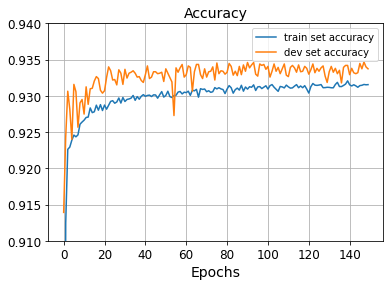
\includegraphics[width=0.5\linewidth]{images/dnn-accuracy-2.png}
\end{center}

After 150 epochs, my DNN model achieved a training set accuracy of 93.18\%, and a development set accuracy of 93.38\%, which is one of the best results of all models I have trained for this task. 

\section{Evaluation}

The test set accuracies of the best of each type of models I have trained for this task are recorded in the following table (as usual, using Dataset 2 (scaled)):

\begin{center}
\begin{tabular}{lr}
\toprule
{} & Test accuracy \\ 
\midrule
Gaussian Naïve Bayes & 57.86\% \\ 
Logistic Regression & 56.02\% \\ 
Single-layer Perceptron & 53.54\% \\ 
\midrule
Hard Voting Classifier & 57.13\% \\
Soft Voting Classifier & 55.34\% \\
\midrule
Bagging Classifier & 79.32\% \\
Pasting Classifier & 79.41\% \\
Random Forest Classifier & 92.14\% \\
AdaBoost Classifier & 91.90\% \\
Gradient Boosting Classifier & 91.01\% \\
\midrule
Deep Neural Network & 93.37\% \\
\bottomrule
\end{tabular} 
\end{center}

The DNN model is the best-performing model in terms of the test set accuracy. The confusion matrix and the precision, recall, F1 scores of the DNN model are shown below:

\begin{center}
\begin{multicols}{2}
\begin{tabular}{lrr}
\toprule
{} & \texttt{1-yes} & \texttt{2-no} \\ 
\midrule
\texttt{1-yes} & 7866 & 608 \\ 
\texttt{2-no} & 570 & 7504 \\ 
\bottomrule
\end{tabular} 

\begin{tabular}{lr}
\toprule
Precision & 92.88\% \\
Recall & 92.88\% \\ 
F1 Score & 92.88\% \\ 
\bottomrule
\end{tabular}
\end{multicols}
\end{center}

This shows that the DNN model performs evenly well on predicting both classes. Unfortunately, since there is no direct way to measure the feature importance in a neural network, the feature importance derived from the random forest classifier were used as reference, since the random forest classifier performs nearly as well as the DNN model. The sorted feature importances are shown in the following table:

\begin{center}
\begin{tabular}{lr}
\toprule
{} & Feature importance \\ 
\midrule
\texttt{colour} & 33.74\% \\
\texttt{location} & 22.35\% \\
\texttt{page} & 14.58\% \\
\texttt{page 1 (main category)} & 13.68\% \\
\texttt{order} & 5.25\% \\
\texttt{day} & 4.74\% \\
\texttt{model photography} & 4.34\% \\
\texttt{country} & 1.32\% \\
\bottomrule
\end{tabular} 
\end{center}

Therefore the colour of the product, \texttt{colour}, is the most important feature for predicting \texttt{price 2}. Following that, the photo location on the webpage, \texttt{location}, page number within the e-store website, \texttt{page}, and the main product category, \texttt{page 1 (main category)}, are also very important features for predicting \texttt{price 2}, compared to the other features.

\section{Visualisation and Dimensionality Reduction}

Firstly, the splom on the Dataset 2 (unscaled) is plotted, with colour-coding by \texttt{price 2}, in order to gain initial insights for further dimensionality reduction:

\begin{center}
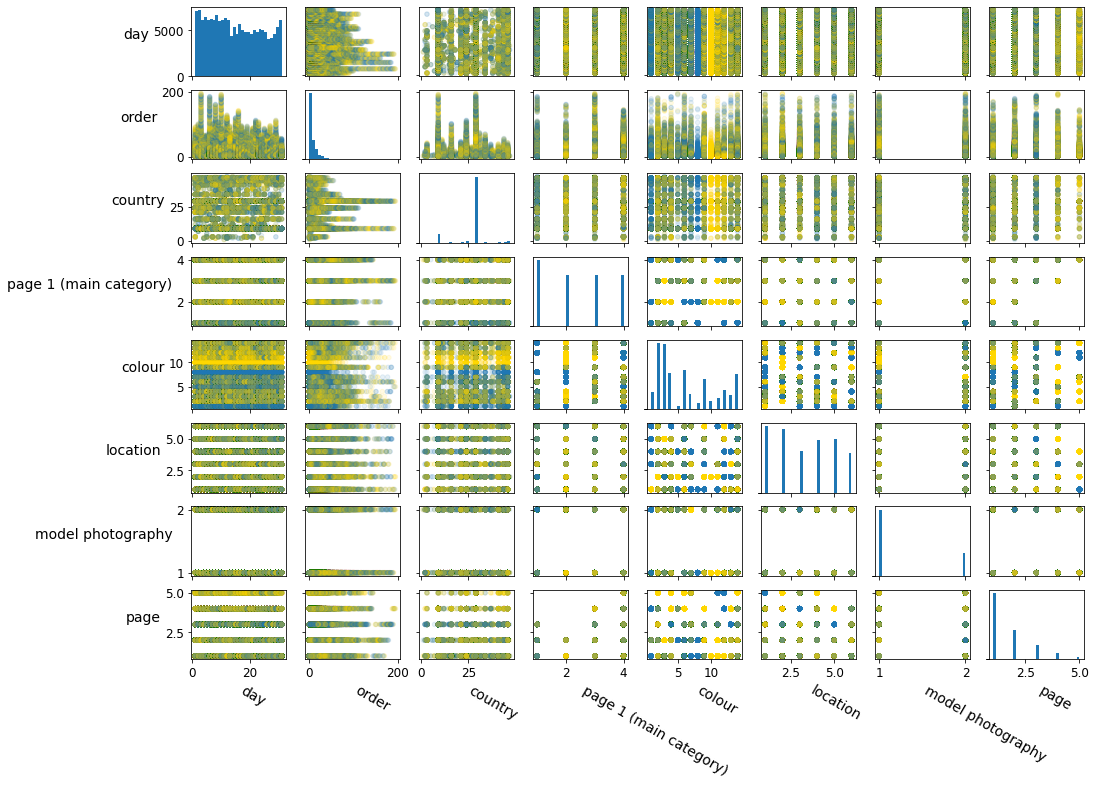
\includegraphics[width=\linewidth]{images/splom.png}
\end{center}

It shows on the splom that there is indeed a notable split on the \texttt{colour} attribute, which cross-validates the feature importance obtained from the previous section. PCA is then applied on Dataset 2 (scaled), and a scatter plot of the first 2 components, which represent the 2 most important features, \texttt{colour} and \texttt{location}, is shown in the below diagram:

\begin{center}
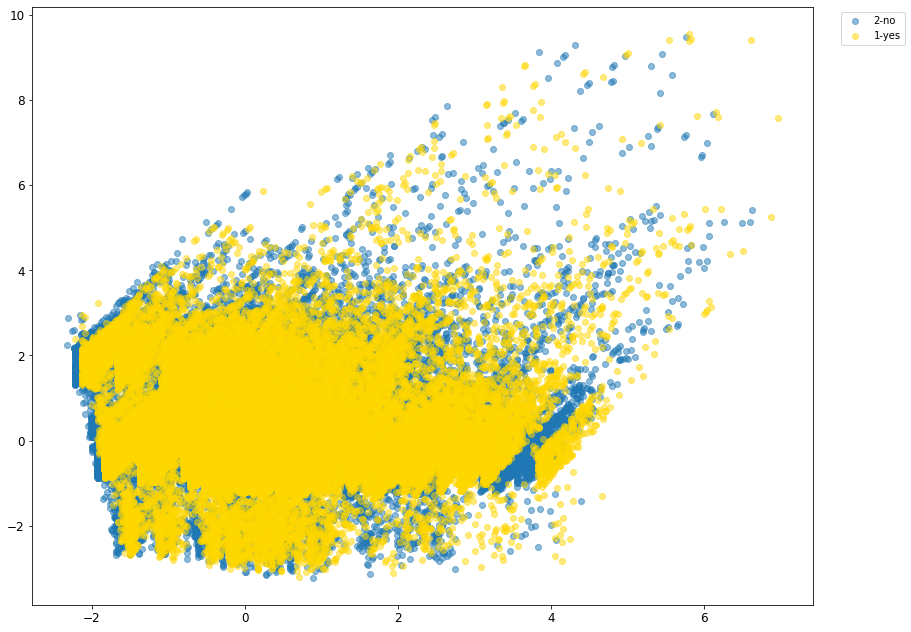
\includegraphics[width=0.6\linewidth]{images/pca.png}
\end{center}

The scatters of the 2 classes almost overlap with each other, which does not provide a helpful clustering for this task. t-SNE is also applied on Dataset 2 (scaled), with different perplexities, and scatter plots of the first 2 components are also plotted, as shown in the following diagrams:

\begin{figure}
    \centering
    \begin{subfigure}[b]{0.49\linewidth}
        \centering
        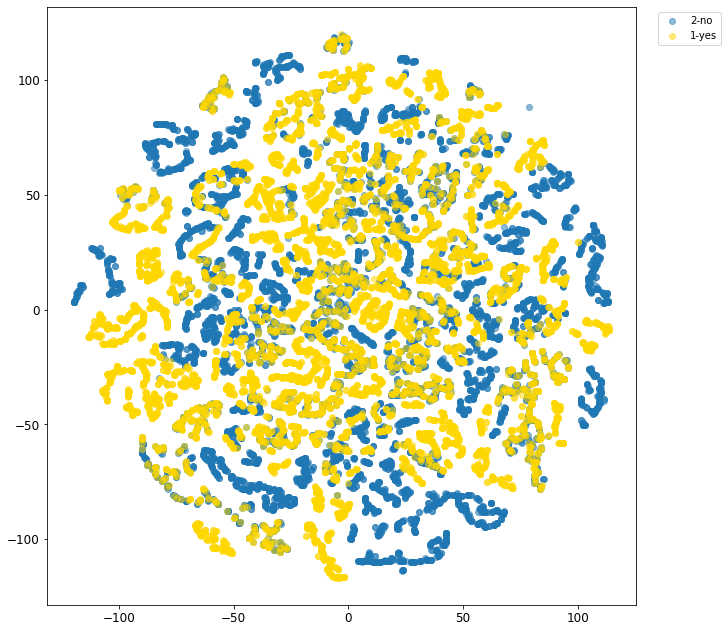
\includegraphics[width=\linewidth]{images/tsne-10.png}
        \caption{\texttt{perplexity=10}}
    \end{subfigure}
    \begin{subfigure}[b]{0.49\linewidth}
        \centering
        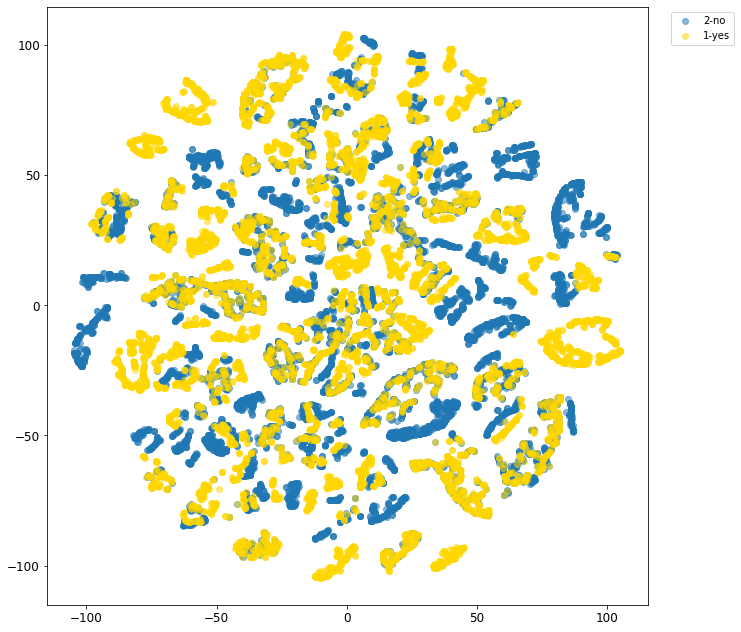
\includegraphics[width=\linewidth]{images/tsne-20.png}
        \caption{\texttt{perplexity=20}}
    \end{subfigure}
    \begin{subfigure}[b]{0.49\linewidth}
        \centering
        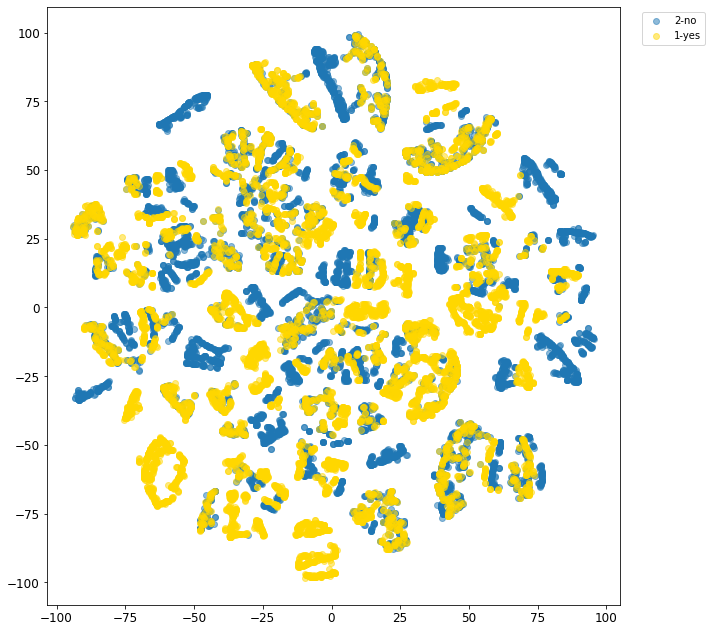
\includegraphics[width=\linewidth]{images/tsne-30.png}
        \caption{\texttt{perplexity=30}}
    \end{subfigure}
    \begin{subfigure}[b]{0.49\linewidth}
        \centering
        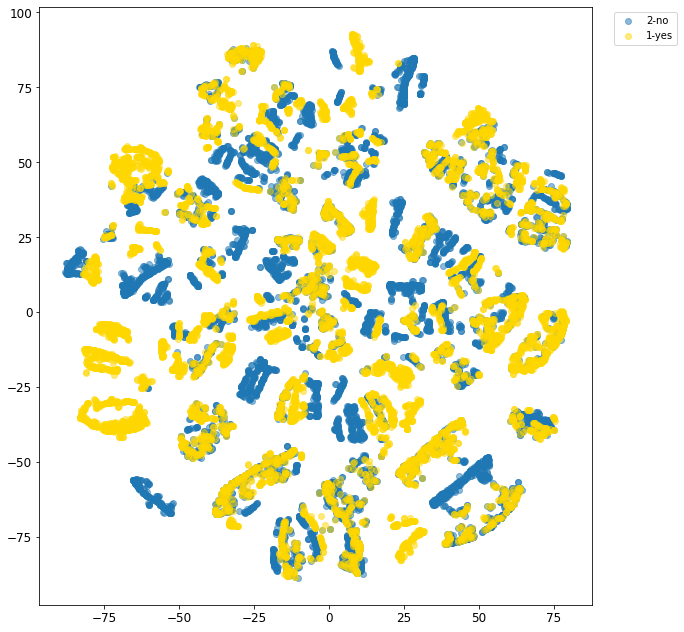
\includegraphics[width=\linewidth]{images/tsne-40.png}
        \caption{\texttt{perplexity=40}}
    \end{subfigure}
    \begin{subfigure}[b]{0.49\linewidth}
        \centering
        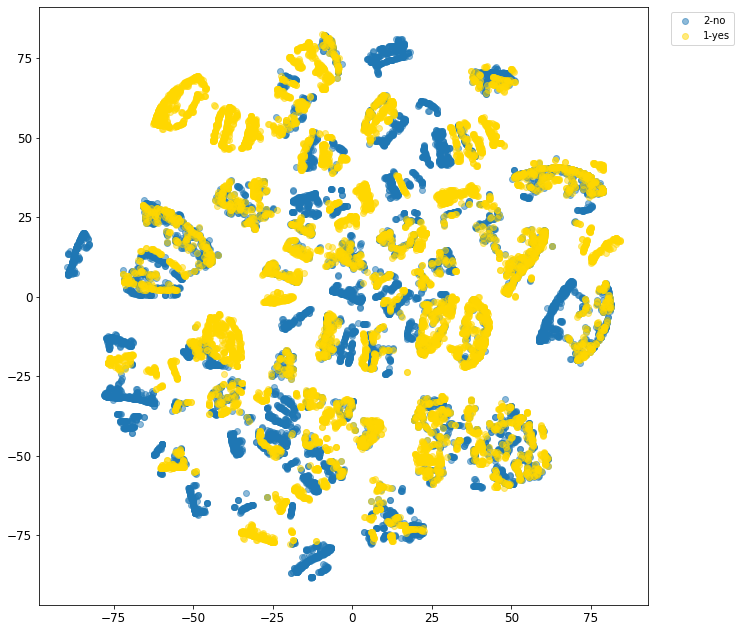
\includegraphics[width=\linewidth]{images/tsne-50.png}
        \caption{\texttt{perplexity=50}}
    \end{subfigure}
\end{figure}

\newpage
t-SNE produces a more helpful clustering visualisation. Also, as the perplexity goes up, the clustering effect becomes more and more notable, and there are less overlapping. This suggests that using t-SNE with a higher perplexity can help more in the visualisation of this task. However, there are still overlaps even when the perplexity is set to 50, which suggests that the 2 most important features alone cannot perfectly separate the two classes, and would have to rely on more features.

\section{Conclusions}

In the final practical, I built various models to predict the target value -- \texttt{price 2}, and achieved a maximum test set accuracy of 93.37\%, using a deep neural network. By inspecting on the data, calculating the feature importances from the models, and cross-validating with various dimensionality reductions, I also found the important features in predicting \texttt{price 2}, which are the colour of the product, \texttt{colour}, and the photo location on the webpage, \texttt{location}.

\bibliographystyle{unsrt}
\bibliography{references}

\end{document}
